\documentclass[journal,12pt,twocolumn]{IEEEtran}

\usepackage{setspace}
\usepackage{gensymb}
\singlespacing
\usepackage[cmex10]{amsmath}

\usepackage{amsthm}

\usepackage{mathrsfs}
\usepackage{txfonts}
\usepackage{stfloats}
\usepackage{bm}
\usepackage{cite}
\usepackage{cases}
\usepackage{subfig}

\usepackage{longtable}
\usepackage{multirow}

\usepackage{enumitem}
\usepackage{mathtools}
\usepackage{steinmetz}
\usepackage{tikz}
\usepackage{circuitikz}
\usepackage{verbatim}
\usepackage{tfrupee}
\usepackage[breaklinks=true]{hyperref}
\usepackage{graphicx}
\usepackage{tkz-euclide}

\usetikzlibrary{calc,math}
\usepackage{listings}
    \usepackage{color}                                            %%
    \usepackage{array}                                            %%
    \usepackage{longtable}                                        %%
    \usepackage{calc}                                             %%
    \usepackage{multirow}                                         %%
    \usepackage{hhline}                                           %%
    \usepackage{ifthen}                                           %%
    \usepackage{lscape}     
\usepackage{multicol}
\usepackage{chngcntr}

\DeclareMathOperator*{\Res}{Res}

\renewcommand\thesection{\arabic{section}}
\renewcommand\thesubsection{\thesection.\arabic{subsection}}
\renewcommand\thesubsubsection{\thesubsection.\arabic{subsubsection}}

\renewcommand\thesectiondis{\arabic{section}}
\renewcommand\thesubsectiondis{\thesectiondis.\arabic{subsection}}
\renewcommand\thesubsubsectiondis{\thesubsectiondis.\arabic{subsubsection}}


\hyphenation{op-tical net-works semi-conduc-tor}
\def\inputGnumericTable{}                                 %%

\lstset{
%language=C,
frame=single, 
breaklines=true,
columns=fullflexible
}
\begin{document}


\newtheorem{theorem}{Theorem}[section]
\newtheorem{problem}{Problem}
\newtheorem{proposition}{Proposition}[section]
\newtheorem{lemma}{Lemma}[section]
\newtheorem{corollary}[theorem]{Corollary}
\newtheorem{example}{Example}[section]
\newtheorem{definition}[problem]{Definition}

\newcommand{\BEQA}{\begin{eqnarray}}
\newcommand{\EEQA}{\end{eqnarray}}
\newcommand{\define}{\stackrel{\triangle}{=}}
\bibliographystyle{IEEEtran}
\raggedbottom
\setlength{\parindent}{0pt}
\providecommand{\mbf}{\mathbf}
\providecommand{\pr}[1]{\ensuremath{\Pr\left(#1\right)}}
\providecommand{\qfunc}[1]{\ensuremath{Q\left(#1\right)}}
\providecommand{\sbrak}[1]{\ensuremath{{}\left[#1\right]}}
\providecommand{\lsbrak}[1]{\ensuremath{{}\left[#1\right.}}
\providecommand{\rsbrak}[1]{\ensuremath{{}\left.#1\right]}}
\providecommand{\brak}[1]{\ensuremath{\left(#1\right)}}
\providecommand{\lbrak}[1]{\ensuremath{\left(#1\right.}}
\providecommand{\rbrak}[1]{\ensuremath{\left.#1\right)}}
\providecommand{\cbrak}[1]{\ensuremath{\left\{#1\right\}}}
\providecommand{\lcbrak}[1]{\ensuremath{\left\{#1\right.}}
\providecommand{\rcbrak}[1]{\ensuremath{\left.#1\right\}}}
\theoremstyle{remark}
\newtheorem{rem}{Remark}
\newcommand{\sgn}{\mathop{\mathrm{sgn}}}
\providecommand{\abs}[1]{\left\vert#1\right\vert}
\providecommand{\res}[1]{\Res\displaylimits_{#1}} 
\providecommand{\norm}[1]{\left\lVert#1\right\rVert}
%\providecommand{\norm}[1]{\lVert#1\rVert}
\providecommand{\mtx}[1]{\mathbf{#1}}
\providecommand{\mean}[1]{E\left[ #1 \right]}
\providecommand{\fourier}{\overset{\mathcal{F}}{ \rightleftharpoons}}
%\providecommand{\hilbert}{\overset{\mathcal{H}}{ \rightleftharpoons}}
\providecommand{\system}{\overset{\mathcal{H}}{ \longleftrightarrow}}
	%\newcommand{\solution}[2]{\textbf{Solution:}{#1}}
\newcommand{\solution}{\noindent \textbf{Solution: }}
\newcommand{\cosec}{\,\text{cosec}\,}
\providecommand{\dec}[2]{\ensuremath{\overset{#1}{\underset{#2}{\gtrless}}}}
\newcommand{\myvec}[1]{\ensuremath{\begin{pmatrix}#1\end{pmatrix}}}
\newcommand{\mydet}[1]{\ensuremath{\begin{vmatrix}#1\end{vmatrix}}}
\numberwithin{equation}{subsection}
\makeatletter
\@addtoreset{figure}{problem}
\makeatother
\let\StandardTheFigure\thefigure
\let\vec\mathbf
\renewcommand{\thefigure}{\theproblem}
\def\putbox#1#2#3{\makebox[0in][l]{\makebox[#1][l]{}\raisebox{\baselineskip}[0in][0in]{\raisebox{#2}[0in][0in]{#3}}}}
     \def\rightbox#1{\makebox[0in][r]{#1}}
     \def\centbox#1{\makebox[0in]{#1}}
     \def\topbox#1{\raisebox{-\baselineskip}[0in][0in]{#1}}
     \def\midbox#1{\raisebox{-0.5\baselineskip}[0in][0in]{#1}}
\vspace{3cm}
\title{EE3025 ASSIGNMENT- 1}
\author{SAI KARTHIK R - EE18BTECH11037}
\maketitle
\newpage
\bigskip
\renewcommand{\thefigure}{\theenumi}
\renewcommand{\thetable}{\theenumi}
Download all python codes from 
\begin{lstlisting}
https://github.com/adi2000pedavegi/ee3025-idp/tree/master/Assignment-1/codes
\end{lstlisting}
%
and latex-tikz codes from 
%
\begin{lstlisting}
https://github.com/adi2000pedavegi/ee3025-idp/tree/master/Assignment-1
\end{lstlisting}
\section{Problem}
    
The command
\begin{lstlisting}
    output_signal = signal.lfilter(b,a,output_signal)
\end{lstlisting}
in Problem 2.3 is executed through following difference equation 
    \begin{align}
        \sum _{m=0}^{M}a\brak{m}y\brak{n-m}=\sum _{k=0}^{N}b\brak{k}x\brak{n-k}
    \end{align}
 where input signal is $x(n)$ and output signal is $y(n)$ with intial values all 0. Replace \textbf{signal.filtfilt} with your own routine and verify
  \section{Solution}
  
  Let $X(z)$ and $Y(z)$ be the respective z-transforms of $x(n)$ and $y(n)$ respectively.
  Using the properties of z-transform
  \begin{align}
      {\mathcal {Z}}\{x(n-k)\} = z^{-k}X(z) \\
      {\mathcal {Z}}\{y(n-m)\} = z^{-m}Y(z)
  \end{align}
\newline
Applying z-transform  to the both sides of the difference equation
\begin{align}
     Y\brak{z} \brak{\sum _{m=0}^{M}a\brak{m} z^{-m}} = X\brak{z} \brak{\sum _{k=0}^{N}b\brak{k}z^{-k}}
\end{align}
\begin{align}
\label{eq:HZ_eqn}
    H\brak{z} = \frac{Y\brak{z}}{X\brak{z}} = \frac{\sum _{k=0}^{N}b\brak{k} z^{-k}}{\sum _{m=0}^{M}a\brak{m}z^{-m}}
\end{align}    
$H(K)$ is evaluated from \eqref{eq:HZ_eqn} using the coefficients b,a.
\\
\\
$X(z)$ is evaluated using a built in fft command, since the manual code written will be of order $O(n^{2})$ where n (length of the given signal) is large. So, it takes too much time.
\\
\\
$Y(z)$ is evaluated by multiplying $X(z)$ and $H(z)$.
\begin{align}
    Y\brak{K} = H\brak{K}X\brak{K}
\end{align}
\\
$y(n)$ is evaluated using a built in ifft command from $Y(z)$ because of the same reason, i.e, manual code written takes too much time
\\
\\
The python code used to obtain the output signal and draw the plots is
\begin{lstlisting}
codes/ee18btech11037.py
\end{lstlisting}
Below is the soundfile constructed from output signal y using own routine filter 
\begin{lstlisting}
codes/Sound_With_ReducedNoise_ownroutine.wav
\end{lstlisting}
\section{Verification}
Both the ouput signals obtained using builtin signal.filtfilt command and own routine method sounds the same.
\\
Plotting the time domain output signal evaluated from both own routine filter and signal.filtfilt command
\begin{figure}[!h]
\centering
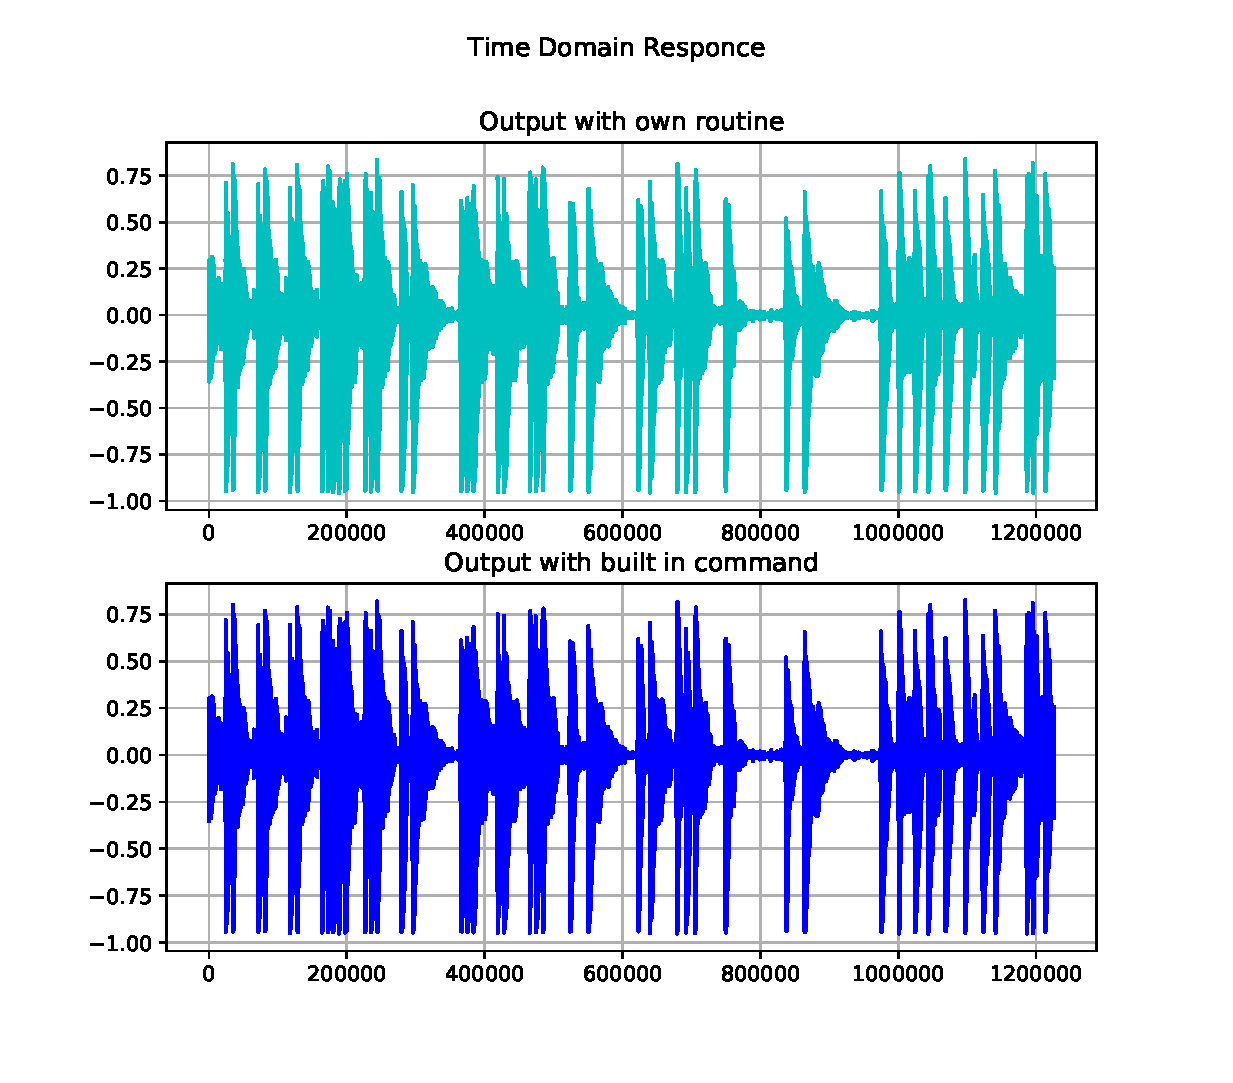
\includegraphics[width=1.2\columnwidth]{figs/ee18btech11037_1.eps}
\caption{Time domain response}
\label{fig:timeresponce}
\end{figure}
\\
Plotting the frequency domain response evaluated from both own routine and signal.filtfilt
\begin{figure}[!h]
\centering
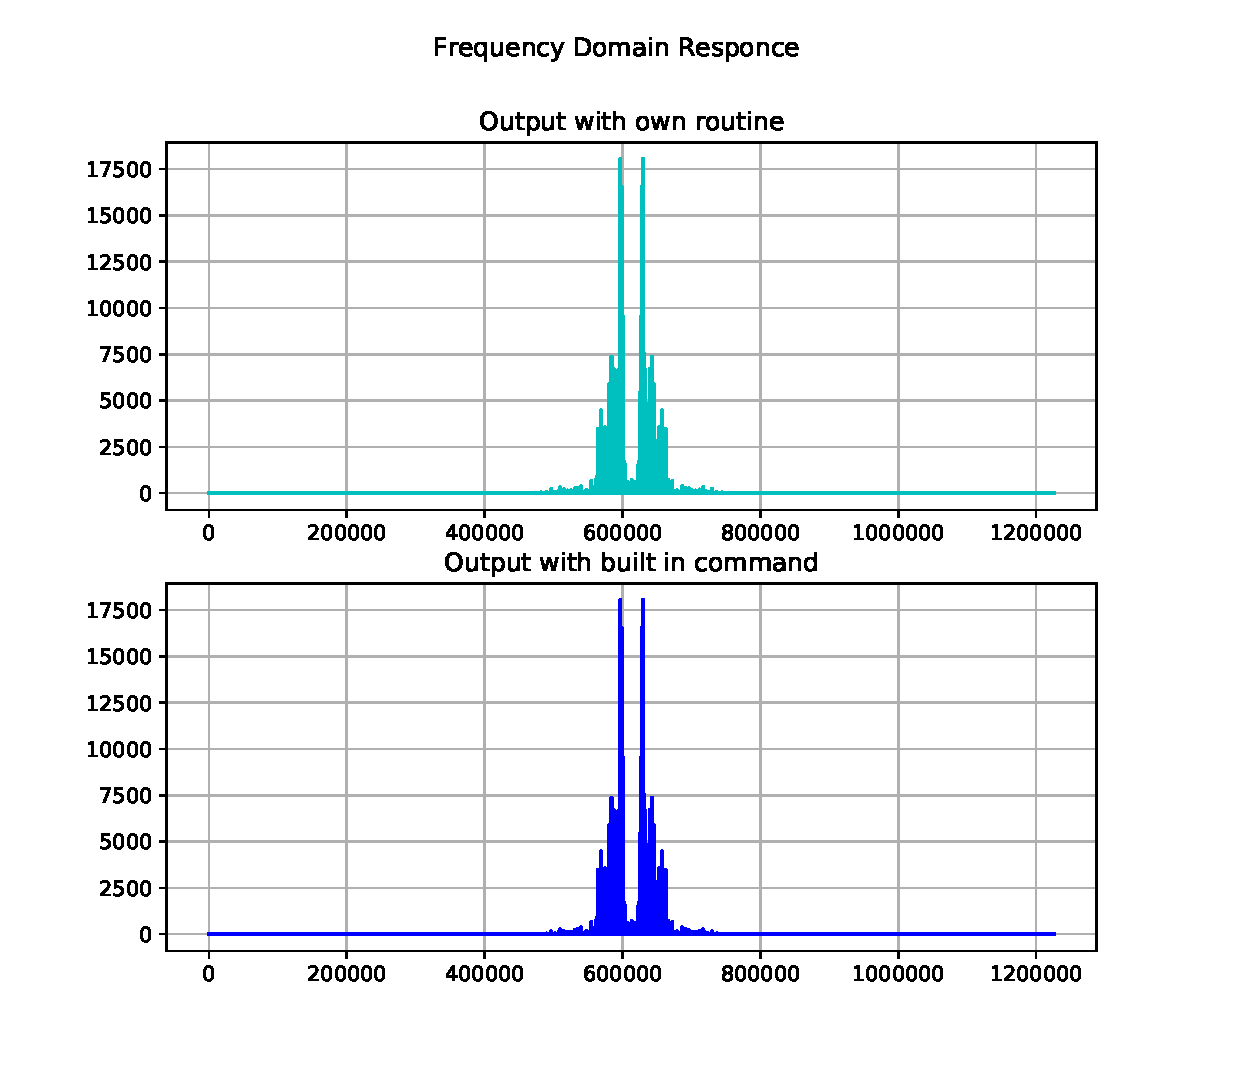
\includegraphics[width=1.2\columnwidth]{figs/ee18btech11037_2.eps}
\caption{Frequency domain response}
\label{fig:freqresponce}
\end{figure}
\end{document}